\documentclass[12pt, a4paper]{scrartcl}

% --packages--
\usepackage[utf8]{inputenc}
\usepackage[italian]{babel}
\usepackage{graphicx}
\usepackage{MnSymbol}
\setlength{\parindent}{0pt}

\title{\textbf{Smart House}}
\author{735722 - Mattia Curatitoli\\ 737838 - Danilo Deponti} \date{}

\begin{document}
\maketitle
 
\section*{Introduzione}
L'invecchiamento della popolazione ha un impatto sempre più significativo sul sistema sanitario. Per questo si cercano vie più efficienti per portare assistenza in casa delle persone bisognose, in particolare gli anziani, il cui numero secondo le stime é in costante aumento grazie alle migliori condizioni di vita e di cure.

Monitorare le attività umane (\texttt{ADL}) è diventato un aspetto fondamentale per costruire un ambiente intelligente atto a garantire il benessere in grado di aumentare sia la sicurezza, sia l'autonomia dei soggetti.

Uno degli approcci più promettenti ed economici è il monitoraggio delle attività tramite una rete wireless di sensori (\texttt{WSN}) disposti nell'ambiente abitativo, in quanto molto flessibile e di facile sviluppo.
Sono stati sviluppati parecchi modelli che utilizzano sensori per monitorare le attività \texttt{ADL}, come ad esempio \emph{Reti Bayesiane} o \emph{Conditional Random Fields}. In particolare, si è notato che \emph{\textbf{Hidden Markov Model (HMM)}} è un modello performante in questo dominio applicativo; alcuni articoli approfondiscono il modello proponendo soluzioni di HMM ibridi, noi invece abbiamo implementato una versione classica.

\section*{I sensori}
Per costruire e testare il modello, sono stati utilizzati dataset presi da due appartamenti. Ogni appartamento fornisce due dataset: il primo con le rilevazioni generate dai sensori, il secondo con le attività rilevate dai sensori.
I sensori utilizzati sono stati di vario tipo (magnetici, a pressione, elettrici etc), disposti in più zone della casa in maniera il meno invasiva possibile e hanno registrato e salvato i dati per diversi intervalli di tempo (due settimane circa).

Il dataset delle rilevazioni sensoristiche (figura \ref{fig:dataset-sensori}) è una lista di righe corrispondenti all'intervallo di tempo nei quali i sensori sono stati attivi. Ogni riga é composta da: 
\begin{center}\begin{addmargin}[2em]{2em}
\texttt{Start time - End time - Location - Type - Place}
\end{addmargin}\end{center}
dove la tripla \texttt{Location-Type-Place} indica il sensore che ha effettuato la rilevazione.
\begin{figure}[!ht]
	\centering
	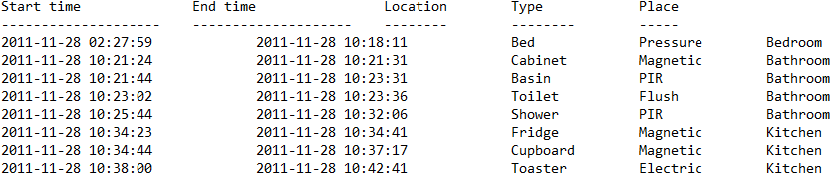
\includegraphics[scale=0.55]{Sensor.png} 
	\caption{Dataset dei sensori}
	\label{fig:dataset-sensori}
\end{figure}

Nel dataset delle attività ogni riga contiene l'intervallo di tempo e il nome dell'attività rilevata. 
Ogni attività è strettamente legata alla rilevazione effettuata dai sensori, ed é rappresentata (figura \ref{fig:dataser-activity}) su una riga come:
\begin{center}\begin{addmargin}[2em]{2em}
\texttt{Start time - End time - Activity}
\end{addmargin}\end{center}
\begin{figure}[!ht]
	\centering
	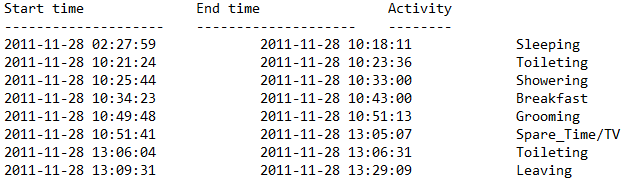
\includegraphics[scale=0.55]{Activity.png} 
	\caption{Dataset delle attività}
	\label{fig:dataser-activity}
\end{figure}

\section*{HMM}
Un \emph{HMM (Hidden Markov Model)} è un modello probabilistico definito da variabili osservabili $x_t$ e variabili nascoste $y_t$, dove $t$ indica il tempo. In questo caso le variabili osservabili sono i sensori, mentre le variabili nascoste sono le attività e dipendono come in figura \ref{fig:dependece-hmm}. 

In un \texttt{HMM} standard le variabili nascoste $y_t$ ($y$ al tempo $t$) dipendono solo dallo stato delle variabili $y_{t-1}$ ($y$ al tempo $t-1$), mentre le variabili osservabili $x_t$ ($x$ al tempo $t$) dipendono solo dallo stato delle variabili $y_t$ ($y$ allo stesso istante $t$).
\begin{figure}[!ht]
	\centering
	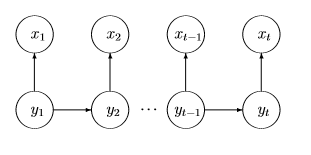
\includegraphics[scale=1]{HMM.png} 
	\caption{Dipendenze in un Hidden Markov Model}
	\label{fig:dependece-hmm}
\end{figure}

Necessari in un \texttt{HMM} sono: 
\begin{itemize}
\item i dati relativi a $p(y)$, ovvero la probabilità a priori delle variabili $y$; 
\item $p(y_t|y{_t-1})$ le probabilità di transizione da uno stato $y$ al successivo; 
\item $p(x_t|y_t)$ le probabilità di una variabile $x_t$ data $y_t$.
\end{itemize}

\section*{Il Software}
Il software è stato sviluppato in \texttt{Python}, e permette di creare un \texttt{HMM} partendo da una sequenza di rilevazioni prese dal dataset di un appartamento. 

Si è deciso di trasformare le rilevazioni dal formato testuale fornito \texttt{.txt} in un formato più compatto ed ordinato, il \texttt{csv}. Come verrà spiegato dettagliatamente nel paragrafo successivo, il software analizza il file e calcola le probabilità iniziali, di transizione degli stati e di emissione degli eventi in base alle occorrenze all'interno del file. Successivamente, il software si avvale di una libreria free di nome \texttt{GHMM}, in grado di creare modelli \texttt{HMM}, fare del \emph{training} su di essi e permette inoltre di inferire sul modello creato.

%Su ogni file sono stati svolti controlli di consistenza sui dati rilevati (se il timestamp di inizio rilevazione è inferiore alla fine, se gli eventi sono temporalmente consecutivi ecc...).
Per la lettura del file dei sensori, la tripla \texttt{Location-Type-Place} è stata utilizzata come chiave univoca per la definizione delle emissioni, che vengono quindi considerate come stati distinti per ogni nuova tripla rilevata all'interno del file.

\section*{Le funzioni}
Di seguito sono descritte le funzioni principali del software, in modo da illustrare dettagliatamente il metodo usato per creare le probabilità utilizzate per la creazione del modello.

\subsection*{check\_and\_generate\_csv}
Prende in input il path di un file testuale \texttt{.txt} ed esamina riga per riga (evitando le prime due che nel dataset fornito sono di intesazione) e per ognuna verifica che lo \texttt{Start time} sia antecedente al \texttt{End time}; sono stati anche implementati, ma non funzionanti, i controlli tra gli \texttt{Start time} e \texttt{End time} tra righe consecutive. Se non sono presenti errori genera un file \texttt{.csv} con i dati controllati, altrimenti lancia un messaggio di errore che indica in quale righe sono state rilevate incorrettezze.

\subsection*{normalize\_list e normalize\_matrix}
Queste funzioni prendono in input rispettivamente liste e matrici e normalizzano i dati contenuti, utilizzando la divisione fornita della libreria \texttt{numpy}. In questo modo ogni lista e ogni riga della matrice ha come somma $1.0$.

\subsection*{csv\_list e csv\_matrix}
Come facilmente intuibile, generano file in formato \texttt{.csv} a partire dai dati in input: lista dei nomi delle variabili (su righe e colonne per la matrice) e lista (o matrice) dei valori da inserire.

\subsection*{obtain\_p\_adls}
Permette di ricavare la lista delle attività rilevate e le probabilità iniziali di ogni singola attività. Questa funzione prende in input il percorso del file csv contenente le attività da analizzare e semplicemente conta le occorrenze di ciascuna stessa attività all'interno del file incrementando un contatore ad ogni rilevazione, dopodichè normalizza i dati.

\subsection*{obtain\_t\_adls}
Permette di ricavare la matrice delle transizioni per le \texttt{ADLs}. Conta, ogni volta che un attività accade al tempo $t$, quante volte ogni singola attività compare al tempo $t-1$, in modo da generare una matrice $n\times n$ con la somma, per ogni attività, delle volte che le altre attività sono accadute successivamente. Infine normalizza i dati.

\subsection*{obtain\_list\_sens}
A partire dal file in input ricava la lista dei sensori attivati durante le rilevazioni (composti dalla tripla univoca \texttt{Location-Type-Place}) e l'elenco con cui sono stati attivati.

\subsection*{obtain\_o\_sens\_adls}






\end{document}
